\documentclass[12pt, letterpaper]{article}

\title{CS302: Trees \color{red}\textbf{[KEY]}\normalcolor}
\author{Amiel L. Iliesi}
\date{2026-04-08}

% packages
\usepackage[hidelinks]{hyperref}
\usepackage[x11names]{xcolor}
\usepackage{graphicx}

% new commands
\newcommand{\question}[1]{\textbf{#1}\par}
\newcommand{\answer}[1]{\color{Green4}\textbf{#1}\normalcolor}

% new environments
\newenvironment{answerblock}{\color{Green4}}{\normalcolor\vspace{1em}}

% global settings
\setlength{\parindent}{0pt}
\setlength{\parskip}{0.5em}
\graphicspath{{./figures/}}

\begin{document}

\maketitle

\tableofcontents

\pagebreak
\section{Trees in General}

\question{In your words, describe a tree. Include all properties that
\emph{all} trees \emph{must} have.}

\begin{answerblock}
A tree is any structure that has nodes which have children. As long as there
are no cycles in the structure, it is a tree.
\end{answerblock}

\question{Describe the following terms: depth, height, balanced, full tree, complete tree.}

\begin{answerblock}
\begin{itemize}
    \item \textbf{depth:} how far down a given node is from the root.
    \item \textbf{height:} how high up a given node is from the furthest
    sub-tree leaf.
    \item \textbf{balanced:} a property a tree has when over half of the nodes
    in the tree are full, IE the tree is guaranteed to have few gaps.
    \item \textbf{full tree:} a state for a tree to be in--when all nodes have
    either no, or all children.
    \item \textbf{complete tree:} the tree is completely packed, and any gaps
    take place on the last row of the tree from left to right. This is useful
    because when serialized, the tree can be fit into a contiguous structure
    like an array. See \textbf{heaps} for a useful example of this.
\end{itemize}
\end{answerblock}

\question{What makes iterating on trees so difficult? What is the solution?}

\begin{answerblock}
Trees are inherently branching and recursive structures. The solution then, is
to search them in the same way, with branching recursion. This way you don't
have to try and backtrack and branch with an iterative loop.
\end{answerblock}

\question{Can you give an example of a most basic type of tree; an unordered,
n-child tree.}

\begin{minipage}{\linewidth}
\begin{answerblock}
Something that doesn't make sense to have be ordered, or limit the number of
children, might be something like a 3D model. You might have a root vertex with
edges that come off of it, and they branch out in whatever direction and number
until the object is complete. No apparent ordering, or limit to number of edges.
\end{answerblock}
\end{minipage}

\pagebreak
\section{Ordered Trees}

\subsection{Properties}

\question{What makes ordered trees different? State their required
properties/invariants.}

\begin{answerblock}
Ordered trees must have the propery that when traversed in order, all children
follow the inequality of their parent. For example, in a binary tree, you would
have \(left < current < right\) for all nodes.
\end{answerblock}

\question{Is the following binary tree ordered? Explain your answer.}

\begin{center}
    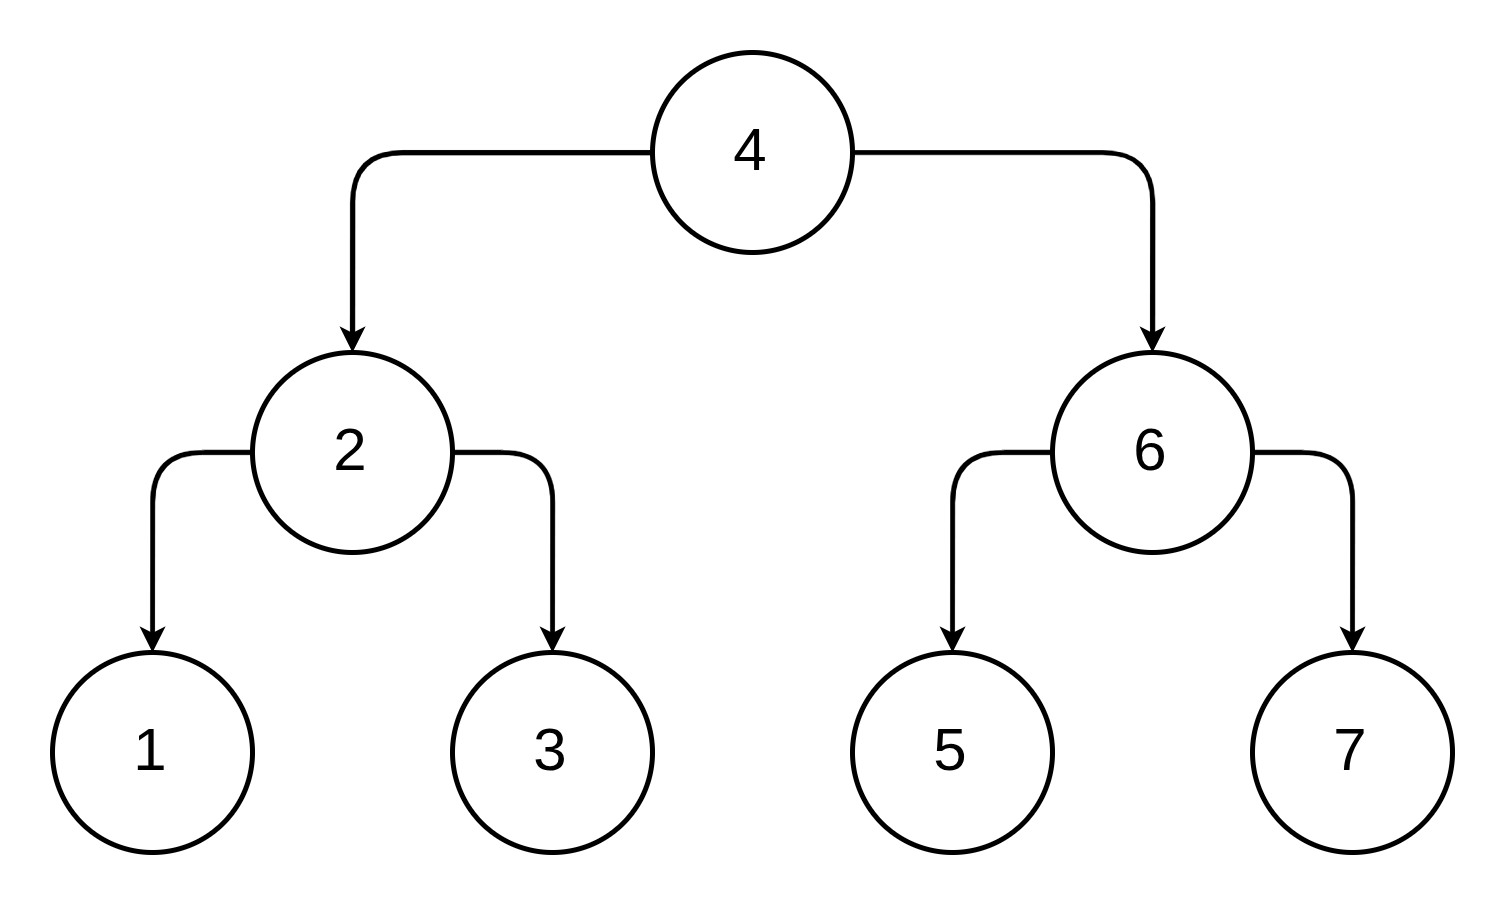
\includegraphics[width=0.5\textwidth]{ordered_tree(1).png}
\end{center}

\begin{answerblock}
Yes, it is ordered. All nodes have no children who violate the expected
ordering.
\end{answerblock}

\begin{minipage}{\textwidth}
\question{Is the following binary tree ordered? Explain your answer.}

\begin{center}
    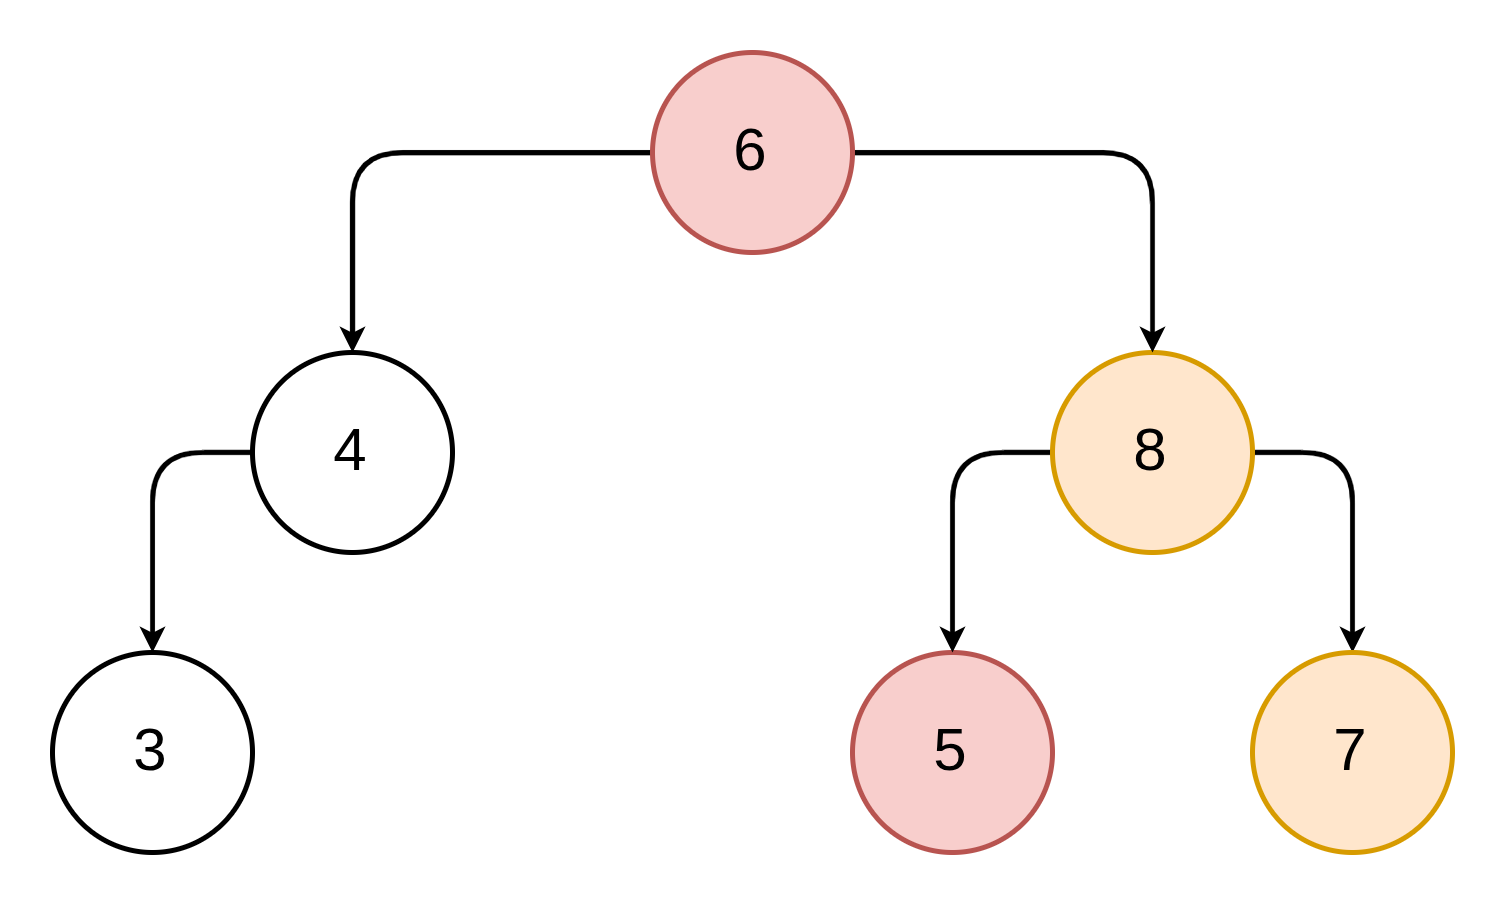
\includegraphics[width=0.5\textwidth]{ordered_tree(2)_highlighted.png}
\end{center}

\begin{answerblock}
No, there are two ordering violations. \(6 < 5\), and \(8 < 7\).
\end{answerblock}

\end{minipage}

\subsection{Implementation}

\question{Describe the process of adding a new integer into an unbalanced,
binary search tree.}

\begin{answerblock}
If you're inserting the first element, it goes uncontested into the root.
Subsequent elements do the following:

If the new node is less than the current node, go left. If the new node is
greater than the current node, go right. When an empty child slot is reached,
the new value is placed there.
\end{answerblock}

\question{Describe the process of removing an integer from an unbalanced,
binary search tree.}

\begin{answerblock}
Search the tree for the value to remove. Recurse left if less, recurse right if
greater. If/when the value is found do one of three things. If the node has no
children, just delete it. If it has one node, swap it with the child then
remove it. If both children exist, then replace it with its in-order successor,
then remove it.
\end{answerblock}

\pagebreak
\section{Balanced vs Unbalanced}

\question{What is a self-balancing tree? Describe a situation where you would
prefer a self-balancing tree, and a situation where you might not prefer one.}

\begin{answerblock}
A self-balancing tree ensures that a tree has roughly equal numbers of nodes in
the left and right side of every given node at all times. It does this with a
specialized structure and/or a specialized insert/remove algorithm.

You usually want this because it bounds the maximum height of the tree, and
resultingly reduces max search time. The only problem is these extra additions
to the structure take time and sometimes memory to perform. If you have a tight
constraint of time or memory, the overhead might be worth considering. Although
there are specialized balanced trees for even those constraints, EG: B-Trees.
\end{answerblock}

\subsection{Types}

\textbf{Describe each of the types below, and what makes them unique. List any
invariants they may have as well.}

\question{Red-Black Tree:}

\begin{answerblock}
Each node is red or black. No red nodes can have red children, and all paths to
root must go through the same number of black nodes. Empty nodes are counted as
black. These constrains ensure that a tree is balanced within a factor of two.
\end{answerblock}

\question{2-3-4 Tree:}

\begin{answerblock}
A node has 2 or 3 values generally, and may have 4 nodes temporarily. This
allows for a specialized splitting and merging which is efficient and
relatively simple, without the slight memory overhead of the red-black tree.
\end{answerblock}

\begin{minipage}{\textwidth}
\question{Heap:}

\begin{answerblock}
Heaps keep things in extrema/height sorted order. The top-level node is
guaranteed to be bigger/smaller than it's children depending on whether the
tree is a min or max heap. Because of that property, with tree-completeness in
mind, can be easily stored into an array, for highly efficient storage and
access. Useful for semi-small data structures that need to be operated on
repeatedly in the CPU.
\end{answerblock}
\end{minipage}

\question{B-Tree:}

\begin{answerblock}
B-Trees are like generalized 2-3-4 trees. The same splitting and merging can be
achieved with any size block, so long as the minimum node storage amount is
half of the max, EG: 2..4, or 50..100. The compacting of nodes allows for
shallower trees, which is super useful if accesses are expensive, EG: cache
misses in a database fetch. This is most data storage and database management
systems use B-Trees at their core.
\end{answerblock}

\end{document}